%% entwurf.tex
%% $Id: entwurf.tex 28 2007-01-18 16:31:32Z bless $
%%

\chapter{Entwurf}
\label{ch:Entwurf}
%% ==============================
In diesem Kapitel erfolgt die ausf{\"u}hrliche Beschreibung des eigenen
L{\"o}sungsansatzes. Dabei sollten L{\"o}sungsalternativen diskutiert und
Entwurfsentscheidungen dargelegt werden.


Bla fasel\ldots

%% ==============================
\section{Programm Ablauf}
%% ==============================
\label{ch:Entwurf:sec:Programm Ablauf}

Bla fasel\ldots

%% Abschnitt1.tex
%% $Id: Abschnitt1.tex 28 2007-01-18 16:31:32Z bless $
%% 3,bischen was

%% ==============================
\section{Ausf{\"u}hrung des Programms}
%% ==============================
\label{ch:Entwurf:sec:Ausf{\"u}hrung des Programms}

Zu Beginn hat man sich {\"u}ber das gesamte Problem einen {\"U}berblick schaffen m{\"u}ssen.
Dabei hat man sich alle einzelnen Bestandteile im Detail angeguckt, um herauszufinden welche Komponenten man wie zusammensetzt. 
Es haben sich drei / vier gro{\ss}e Komponenten ergeben, die man erledigen musste. 

Zuerst habe man sich mit dem Wearable auseinandergesetzt, um zu bestimmen, was man alles mit dem Wearable umsetzen kann.
Man fand dabei heraus, dass man zwei Parameter hatte, die man einstellen konnte. Diese waren die Zeit, wie lang das Wearable vibriert und die St{\"a}rke, wie stark das Armband vibriert.
%Man fand heraus, dass man die Zeit, wie lang das Armband vibriert, und die St{\"a}rke, wie Stark das Armband vibrieren kann, einstellen konnte.
Um ein Signal zu {\"u}bertragen hatte man eine Beschr{\"a}nkung von 20 Bytes, die man maximal in einer Nachricht mittels Bluetooth {\"u}bertragen kann.

Als n{\"a}chste Komponente des Problems habe man sich eine geeignete Repr{\"a}sentation eines Signals {\"u}berlegen m{\"u}ssen. Um nicht au{\ss}er Bedacht zu lassen ist diese die wichtigste Komponente des Problems, denn es h{\"a}ngen alle anderen Komponenten davon ab, wie diese Daten repr{\"a}sentiert werden. 

Daher stellte sich die Frage, wie sieht ein solches Signal aus?

%% ==============================
\subsection{Signal}
%% ==============================

Anhand der zwei Parameter, die L{\"a}nge und die St{\"a}rke des Wearables, hat man diese als Attribute eines Signals definiert.  

Technisch gesehen h{\"a}tte man f{\"u}r die L{\"a}nge eines Signals von 0 ms (0x0000) bis 65535 ms (0xFFFF) nutzen k{\"o}nnen. 
Man hat sich jedoch anhand vorheriger Studien \cite{pescara2016ruttelflug} orientiert und ein Minimum von 100 ms und ein Maximum von 1000 ms als Grenzen f{\"u}r die L{\"a}nge {\"u}bernommen.

Bei der St{\"a}rke eines Signals hat man sich auch hier am Wearable orientiert. 
Die Repr{\"a}sentation der St{\"a}rke musste man aus technischen Gr{\"u}nden ab einem Wert von 32767 (0x7FFF) definieren. Dies war n{\"a}mlich der Wert, ab dem beide Traktoren angefangen haben sp{\"u}rbar, als Vibrationen wahrgenommen zu werden.
%Theoretisch gesehen h{\"a}tte man die gleichen Grenzen von 0 bis 65535 zur Repr{\"a}sentation der St{\"a}rke vorhanden, aber technisch hat man erst ab einer St{\"a}rke von 32767 (0x7FFF) ein sp{\"u}rbare Vibration gehabt. 
Vor dem genannten Wert ist zu wenig Strom {\"u}bertragen worden, sodass kein Traktor funktionierte.
Daher hat man sich zwischen den Grenzen von (0x7FFF) und (0xFFFF) f{\"u}r die St{\"a}rke festgelegt. 

Anhand der Hypothese der Bachelorarbeit wolle man wissen, wie gut sich personalisierte Vibrationen im Vergleich zu generischen Vibrationen verbessern. Dabei musste man sich {\"u}berlegen, wie man personalisierte Vibrationen mittels dem EA f{\"u}r einen Probanden bestimmen will.
Au{\ss}erdem sollte man herausfinden, was f{\"u}r Signale noch gut voneinander unterscheidbar sind, die die Grenzen von 100ms bis 1000ms besitzen.
Man habe sich auf drei Typen von Signalen festgelegt: \textbf{Kurz}, \textbf{Mittel} und \textbf{Lang}. Dadurch wolle man wissen, wie ein Signal wahrgenommen wird und welchen Typen man dem Signal zuordnen w{\"u}rde.

Die jeweiligen Typen definieren innerhalb der Grenzen zwischen 100 ms und 1000 ms ein Intervall, die sich nicht {\"u}berschneiden. Abgesehen davon ist \textbf{kurz}, das zahlenwertig kleinste Intervall, gefolgt von \textbf{mittel}, \textbf{lang} ist das zahlenwertig gr{\"o}{\ss}te Intervall.
Allerdings wurde es darauf geachtet, dass die Grenzen nicht aufeinander liegen, sondern einen Abstand zwischen den Grenzen existiert.
Als Beispiel habe man f{\"u}r Kurz die Intervallgrenzen 100ms und 300ms, f{\"u}r Mittel habe man dann die Intervallgrenzen von 400ms bis 600ms und f{\"u}r Lang habe man die Intervallgrenzen von 700ms bis 1000ms. 

F{\"u}r die St{\"a}rke der Vibration war man an den Darstellbarkeit des Wearables gebunden. Zwischen die Grenzen von (0x7FFF) und (0xFFFF) hat man sich f{\"u}nf voneinander unterscheidbare Stufen definiert.


%Zu Beginn musste man sich {\"u}ber alles einen {\"U}berblick schaffen. 
%Das heißt, dass man sich alle Bestandteile einzeln betrachten musste bevor man alles zusammen setzen konnte. 
%Es gibt drei / vier gro{\ss}e Bestandteile die ich mir {\"u}berlegen musste.

%Zualler erst musste man sich mit dem Armband besch{\"a}ftigen, um herauzufinden, was es alles konnte. 
%Man konnte die Zeit, die das Armband vibrieren sollte festlegen, sowie auch die St{\"a}rke, wie Stark das Armband vibrieren sollte. 
%Man musst darauf achten, dass man die 20 Bytes, die man lediglich mit Bluethooth {\"u}bertragen konnte nicht {\"u}berschreitet.

%Als n{\"a}chstes habe ich mir erst einmal {\"u}berlegt, wie ich die Daten repr{\"a}sentieren sollte. 
%Ich habe mir {\"u}berlegt, dass ich eine Datenstruktur erstellen m{\"u}sste um das Signal anschlie{\ss}end {\"u}ber BLE an das Armband zu {\"u}bertragen. 
%Aber wie sehen Signale aus? 
%Zuerst habe ich mir {\"u}berlegt, was ist die Maximale und Minimale L{\"a}nge, die ich {\"u}bertragen werde. 

%Dabei habe ich mich f{\"u}r einen Minimalen Wert von 100 Millisekunden (ms) und eine Maximale L{\"a}nge von 1024 ms entschieden. 
%Da man das Armabnd auch in verschiedenen Vibrationsst{\"a}rken abspielen konnte, habe ich herausgefunden, manche Vibrationsst{\"a}rken gar keine Vibration abspielten, weil so wenig Strom{\"u}bertragen wurde, dass die Vibrationsmotoren gar nicht erst angesteuert wurden. 
%Dabei haben sich die Grenzen hierbei von 0x7FFF bis 0xFFFF behandelt. 

%Um jedoch merkbare unterschiede der Vibrationsst{\"a}rke zu bestimmen habe ich mir die Grenzen in 5 Bereiche aufgeteilt. 
%Somit hatte ich zwei Variablen, die ich f{\"u}r meine Darstellung von einem Signal entscheidend war. 

%Da ich jetzt Signale mit einer L{\"a}nge von 100 ms bis 1024 ms hatte musste ich mir {\"u}berlegen, wie viele Signaltpyen ich hier erzeugen w{\"u}rde. Der Morsecode beispielsweise bestand aus 3 Teilen ein Kurzes Signal, ein Langes Signal und einer Pause. Dabei wollte ich jetzt nicht den Morsecode nehmen und habe mich f{\"u}r eine eigene Definition entschieden. Dabei habe ich gesagt dass es drei Signaltypen gibt. Diese drei Signaltypen sind Kurz, Mittel und Lang, auf die ich gleich noch einmal zu sprechen komme.

%Vorher will ich auf den Evolution{\"a}ren Algorithmus zu sprechen kommen. 
%Beim Evolution{\"a}ren Algorithmus musste man sich zu beginn eine Anfangspopulation erstellen. 
%Also in meinem Fall w{\"a}re die Anfangspopulation eine Menge von Signalen die eine Variation aufweisen sollte. 




%-----------------
%Wie sollte eine solche Population aussehen? 
%Hier ist mir der Gedanken gekommen, man sollte die Signaltypen in Grenzen aufteilen, das bedeutet, dass man beispielsweise von 100 bis 300 ms Kurz, von 400 bis 700 ms Mittel und von 800 bis 1024 ms Lang definieren sollte. 
%Am Anfang habe ich dies auch gemacht, dass die Grenzen fest von mir vorgegeben waren, jedoch  hat man festgestellt, dass die Nutzer nicht genau diese Grenzen als Kurz, Mittel und Lang empfunden haben. Das hei{\ss}t man musste sich vor dem Evolution{\"a}ren Algorithmus {\"u}berlegen, wie die Nutzer die Signalgrenzen selbst bestimmten. (N{\"a}here Information im Kapitel Implementierung)

%Nach der Bestimmung der Signaltypen, hat man sich erneut an den Evolution{\"a}ren Algorithmus gewagt. Das bedeutete, man musste eine Anfangspopulation bestimmen. Dabei hat man N Individuen f{\"u}r jeden Signaltypen innerhalb seiner Grenzen erzeugt. Zuerst komplett zuf{\"a}llig innerhalb der Grenzen, dabei kam man zu dem Ergebnis, dass die Grenzen nur in seltenen f{\"a}llen drinnen waren. D.h. dass man nie den vollst{\"a}ndigen Intervall den man vorher bestimmt hat in der Anfangspopulation vertreten war. Deshalb habe man von den N Individuen zwei Individuen erzeugt, die genau die beiden Grenzen repr{\"a}sentiert haben.

%Nach der Erzeugung der Anfangspopulation sollten die Signale vom Benutzer alle bewertet werden. 
%Dabei hatte man den Gedanken, dass man den Benutzer die Signale mehrmals abspielt und ihn jedes mal abfragt, was f{\"u}r ein Signal er erkannt hat und anhand der H{\"a}ufigkeit, die er das Signal als den Signaltypen erkannt hat wie das Programm es f{\"u}r Ihn im Vorfeld bestimmt hatte, einen Fittnesswert bestimme. Jedoch m{\"u}ssten diese 3*N Signale mehrmals abgespielt werden, um eine H{\"a}ufigkeit zu erhalten. Wenn man hier f{\"u}r die Population jedes Individuum f{\"u}nf mal abspielen w{\"a}rde, w{\"a}re man bei 15*N. Bei einem N von 10 Signalen pro Signaltyp w{\"a}ren dass dann 150 Bewertungen die der Nutzer pro Population machen m{\"u}sste um nur eine Generation zu bewerten. Wenn man nur vier Generationen bestimmen wollte, so wäre man bei 450 Bewertungen nur um einen personalisierten Wert zu erhalten. Das w{\"a}re f{\"u}r einen normalen Benutzer nicht zumutbar, dass er so viel Zeit in Anspruch nehmen w{\"u}rde um so viele Signale zu bewerten. 

%Daher musste eine alternative her. Die Alternative ist gewesen, man spiele dem Benutzer jedes Individuum nur einmal ab und stellt Ihn dazu drei Fragen, die wie in einem SUS Fragebogen gestellt wird, mit einer Skala von sehr gut bis sehr schlecht. [BILD EINFÃœGEN]
%Anhand der Fragen habe ich einen Fitnesswert bestimmt. Die weitere Beschreibung des Algorithmus wird in der Implementierung beschrieben.

%Mit jeder Generation ist man davon ausgegangen, dass die Grenzen der Signaltypen kleiner wurde und zu dem Wert, dass dem Nutzer am besten gefallen w{\"u}rde hinkonvergieren w{\"u}rde.
 %W{\"u}rde man dies weitertreiben, bis die jeweiligen Signaltypen gegen eine Zahl konvergieren, w{\"u}rde man noch ein paar mehr Itterationen machen m{\"u}ssen, was unter Bedacht, dass der Benutzer nicht so lange die Signale bewerten w{\"u}rde nach vier Itterationen aufgeh{\"o}rt. Nachdem der Algorithmus also nach der vierten Generation die Population erzeugt hat, wurde von allen Individuen das Minumin und Maximum der jeweiligen Signaltypen bestimmt worden. Anhand der Minima und Maxima wurde f{\"u}r jeden Signaltypen der Mittelwert bestimmt.

%Somit hat man nach dem Algorithmus einen personalisierten Kurz, Mittel und Lang Wert.

%Im dritten Schritt musste man herausfinden, wie die Signale im Vergleich zu Vorgegebenen Werten erkannt werden.
%Dabei hat man verschiedene Folgen von Signalen vordefiniert, die der Benutzer erkennen sollte. Dabei habe man zuerst drei Signal-Folgen (aka Muster) abgespielt, anschlie{\ss}end vierer Muster und zu letzt f{\"u}nfer Muster. Es wurde abwechselnd ein zuf{\"a}lliges genetisches Muster und ein generisches Muster abgespielt. 



%% ==============================
\section{Evolutionaerer Algorithmus}
%% ==============================
\label{ch:Entwurf:sec:Evolutionaerer Algorithmus}

%% Abschnitt1.tex
%% $Id: Abschnitt1.tex 28 2007-01-18 16:31:32Z bless $
%%


%% ==============================
\section{Signal}
%% ==============================
Ein Signal bildet eine Vibration ab. Dabei besitzt ein Signal Attribute, die die obengenannte Reaktion darstellen sollten. Als man sich die Einstellungsm{\"o}glichkeiten einer Vibration des Wearable genauer angeguckt hat, hat man festgestellt, dass man die L{\"a}nge und die St{\"a}rke einer Vibration einstellen kann. Das hat zur Folge, dass diese zwei Faktoren als die Attribute eines Signales benutzt wurden um eine Vibration zu repr{\"a}sentieren.

Man stellt sich jetzt die Frage,
Wie lang sollen die Vibrationen denn jetzt sein ? 

Um diese Frage zu beantworten, guckt man sich anhand an dem Paper \cite{pescara2016ruttelflug} die benutzten Vibrationsl{\"a}ngen an. Da wurden die Grenzen zwischen 100 und 1000ms f{\"u}r eine Vibration benutzt. Diese Werte hat man so {\"u}bernommen. Das bedeutet, ein Signal hat eine minimale L{\"a}nge von 100ms und eine maximale L{\"a}nge von 1000 ms. 

Anhand der Hypothese der Bachelorarbeit wolle man wissen, wie gut sich personalisierte Vibrationen im Vergleich zu generischen Vibrationen verbessern. Diese Frage l{\"a}sst sich wie folgt beantworten. Erstens musste man sich {\"u}berlegen, wie man personalisierte Vibrationen mittels dem EA f{\"u}r einen Probanden bestimmen will.
Au{\ss}erdem sollte man herausfinden was f{\"u}r Signale noch gut voneinander unterscheidbar sind, die die Grenzen von 100ms bis 1000ms besitzen.
Man habe sich auf drei Typen von Signalen festgelegt, die als Kurz, Mittel und Lang definiert. Dadurch wolle man wissen, ob ein Signal als Kurz, Mittel oder Lang empfunden wurde.

Die jeweiligen Typen definieren innerhalb der Grenzen von 100ms und 1000ms ein Intervall, das sich voneinander nicht {\"u}berschneiden kann. Abgesehen davon ist der niedrigste Messwert von Lang Signal allgemein gr{\"o}{\ss}er als der h{\"o}chste Messwert von Mittel Signal. Wiederum ist die kleinste Intensit{\"a}t von Mittel Signal ist in der Regel gr{\"o}{\ss}er als die gr{\"o}{\ss}te Internsit{\"a}t von Kurz Signal. Als Beispiel habe man f{\"u}r Kurz die Intervallgrenzen 100ms und 300ms, f{\"u}r Mittel habe man dann die Intervallgrenzen von 400ms bis 600ms und f{\"u}r Lang habe man die Intervallgrenzen von 700ms bis 1000ms. 
Allerdings wurde es darauf geachtet, dass die Grenzen nicht aufeinander liegen, sondern einen Abstand zwischen den Grenzen existiert. Bei der St{\"a}rke einer Vibration wurde man an der Darstellbarkeit des Wearable gebunden. Nachdem man herausgefunden hat, dass man nur die Bereiche von 0x7FFF bis 0xFFFF als merkbare Vibrationsst{\"a}rken besitzt, hat man sich diese Bereiche in 5 Stufen eingeteilt. Daraus folgt dass man sich f{\"u}r den sp{\"a}teren Verlauf f{\"u}nf Zust{\"a}nde definiert. Ein 

\begin{tabular}{lcr}
  Signalst{\"a}rke & Namen & Zustandsnamen \\
  $\mathtt{0x7FFF}$ & Very Weak & $q_{VWeak}$ \\
  $\mathtt{0x9FFF}$ & Weak & $q_{Weak}$ \\
  $\mathtt{0xBFFF}$ & OK & $q_{OK}$ \\
  $\mathtt{0xDFFF}$ & Strong & $q_{Strong}$ \\
  $\mathtt{0xFFFF}$ & Very Strong & $q_{VStrong}$ \\
\end{tabular}


%% ==============================
\section{Muster}
%% ==============================
Ein Muster ist dabei eine Folge von mehreren Signalen.

%% ==============================
\section{Eingabe f{\"u}r den Algorithmus}
%% ==============================
Als Eingabe f{\"u}r den Algorithmus ben{\"o}tigt man eine Population von Individuen. Die Individuen sind in diesem Fall Signale. 
Nicht jede Person empfindet ein vorgegebenes Kurzes Signal gleich wie eine andere Person, somit musste man zuvor den Benutzer befragen, was er als Kurz, Mittel und Lang empfindet. Zuerst habe man alle Signale abgespielt, damit der Proband wusste, was Ihn erwartet. 
Nachdem alle Signale abgespielt wurden, wurde jedes Signal einzeln abgespielt und der Proband hatte die Aufgabe das abgespielte Signal der Kategorie Kurz, Mittel oder Lang zuzuordnen. 
Jedem Probanden wurde insgesamt 10 Signale mit der gleichen Vibrationsst{\"a}rke abgespielt, die Signalel{\"a}nge ist dabei gleich verteilt.
Dabei wurden alle 10 Signale in einer zuf{\"a}lligen Reihenfolge abgespielt.

Nach der Eingabe des Probanden erh{\"a}lt man beispielsweise folgende Bewertung. Diese Eingabe ist ideal, da alle Signaltypen direkt hintereinander vorliegen, so w{\"u}rde man hier ein die Grenzen sofort aus der Tabelle entnehmen k{\"o}nnen. Diese belaufen sich f{\"u}r Kurz zwischen 100 und 300 ms, f{\"u}r Mittel zwischen 400ms und 600ms und f{\"u}r Lang zwischen 700 und 1000ms.

\begin{table}[]
\centering
\caption{My caption}
\label{my-label}
\begin{tabular}{|l|l|l|l|l|l|l|l|l|l|l|}
\hline
 Signall{\"a}nge & 100ms & 200ms & 300ms & 400ms & 500ms & 600ms & 700ms & 800ms & 900ms & 1000ms \\ \hline
 Erkannten Signaltyp & Kurz & Kurz & Kurz & Mittel & Mittel & Mittel & Lang & Lang & Lang & Lang \\ \hline
\end{tabular}
\end{table}

Falls die Eingabe jedoch nicht so Ideal sein sollte, wie in dem Beispiel gerade eben, mussten ein paar Vorkehrungen getroffen werden. Um einige Sonderf{\"a}lle auszuschlie{\ss}en, hat man {\"u}berpr{\"u}ft, ob das Signal mit der L{\"a}nge von 100ms ein Kurzes Signal ist und das Signal mit der L{\"a}nge von 1000ms ein Langes Signal ist, sowie man annimmt, dass mindestens jeder Signaltyp mindesten zwei mal ausgew{\"a}hlt wurde. Sollte dies nicht der Fall sein, so w{\"u}rde man den Benutzer dazu bitten, die zehn Signale erneut zu bewerten. 

\begin{table}[]
\centering
\caption{My caption}
\label{my-label}
\begin{tabular}{|l|l|l|l|l|l|l|l|l|l|l|}
\hline
 Signall{\"a}nge & 100ms & 200ms & 300ms & 400ms & 500ms & 600ms & 700ms & 800ms & 900ms & 1000ms \\ \hline
 Erkannten Signaltyp & Kurz & Kurz & Mittel & Mittel & Lang & Mittel & Lang & Lang & Lang & Lang \\ \hline
\end{tabular}
\end{table}

Man beginnt damit die neuen Intervallgrenzen zu bestimmen. Diese wurden anhand des Beispiels exemplarisch in der Tabelle bestimmt, dabei ist jede Spalte eine Itteration.

\begin{table}[]
\centering
\caption{My caption}
\label{my-label}
\begin{tabular}{|l|l|l|l|l|l|l|l|l|l|}
\hline
Itterationen            & 1. & 2. & 3. & 4. & 5. & 6. & 7. & 8. & 10. \\ \hline
$Kurz_{Min}$   & 100          & 100          & 100          & 100          & 100          & 100          & 100          & 100          & 100           \\ \hline
$Kurz_{Max}$   & 100          & 200          & 200          & 200          & 200          & 200          & 200          & 200          & 200           \\ \hline
$Mittel_{Min}$ & 100          & 200          & 300          & 300          & 300          & 300          & 300          & 300          & 300           \\ \hline
$Mittel_{Max}$ & 100          & 200          & 300          & 400          & 400          & 600          & 600          & 600          & 600           \\ \hline
$Lang_{Min}$   & 100          & 200          & 300          & 400          & 500          & 600          & 700          & 700          & 700           \\ \hline
$Lang_{Max}$   & 100          & 200          & 300          & 400          & 500          & 600          & 700          & 800          & 1000          \\ \hline
\end{tabular}
\end{table}

Bei einer kleinen Abweichung von zwei nebeneinanderliegen von zwei Werten ist dies noch akzeptabel, bei gr{\"o}{\ss}eren Abweichungen, hat man Benutzer noch einmal darum gebeten erneut zu bewerten. Im Verlauf der Studie musste man nur bei einer Minderheit von Probanden ein weiteres mal darum bitten, die Signale neu zu bewerten. Denn es ist oft schon so gewesen, dass die Probanden es wie im Idealfall zugeordnet hatten.

\begin{comment}
Anhand dem Verfahren hat man nur eine grobe Unterteilung, deswegen {\"u}berpr{\"u}ft man, ob diese grobe Absch{\"a}tzung passt.
Zun{\"a}chst bestimmt man f{\"u}r jeden Signaltypen das arithmetische Median, was in diesem Fall 150 f{\"u}r Kurz, 433 f{\"u}r Mittel und 780 f{\"u}r Lang ist.
Da sich die Grenzen vom Minimum von Kurz und das Maximum von Lang nicht {\"a}ndern, sind $Kurz_{Min}$ = 100ms und $Lang_{Max}$ = 1000ms bei jedem Probanden fest definiert und beginnt damit f{\"u}r Kurz und Lang die Grenzen zu bestimmen.
Zuerst berechnet man anhand der groben Absch{\"a}tzung der Grenzen den Mittelwert, dabei ergibt sich $Kurz_{Mit}$ = 150 und $Lang_{Mit}$ = 850.

Wenn das arithmetische Median kleiner als der Mittelwert ist, dann berechnet man bei Kurz ein neues Maximum und bei Lang ein neues Minimum.
Bei Kurz ist dies nicht der Fall, da der Median und Mittelwert beide 150 sind, daher bleibt $Kurz_{Max}$ = 200ms.
Bei Lang tritt dieser Fall ein und daher berechnet anhand der Formel $Lang_{Min} = (2 * Lang_{Med}) - Lang_{Max}$ daraus ergibt sich f{\"u}r $Lang_{Min}$ = 560. 

W{\"u}rden sich die erkannten Signaltypen {\"u}berschneiden, so f{\"a}ngt man an das arithmetische Mittel von Kurz, Mittel und Lang zu bilden; desweiteren werden neue Grenzen bestimmt, indem man von der kleinsten Signall{\"a}nge anf{\"a}ngt und diese dann dem zuwei{\ss}t, was ausgew{\"a}hlt worden ist. Man hat drei mal das Minimum und das Maximum von Kurz, Mittel und Lang, die neu bestimmt werden, dabei wird anhand der folgenden Tabelle gezeigt, wie die neuen Intervalle bestimmt werden.


Da man wei{\ss}, dass das Minimum von Kurz 100ms und das Maximum von Lang 1000ms ist, berechnet man die Intervalle von Kurz und Lang zuerst. Dabei berechnet man den Mittelwert um herauszufinden, ob das arithmetische Mittel identisch mit dem Mittel wert ist. Wenn dies der Fall ist, so sind die Grenzen f{\"u}r den Fall richtig und es muss f{\"u}r den Signaltypen nichts weiter berechnet werden. 

Da man wei{\ss}, dass das Minimum von Kurz 100 ms und das Maximum von Lang 1000ms ist, berechnet man die Differenz zwischen dem  und dem Minimum von Kurz. Diese Differenz auf das Median dazu addiert und {\"u}berpr{\"u}ft, ob 
\end{comment}

\usepackage{pgf}
\usepackage{tikz}
\usetikzlibrary{arrows,automata}
\usepackage[latin1]{inputenc}
\usepackage{verbatim}


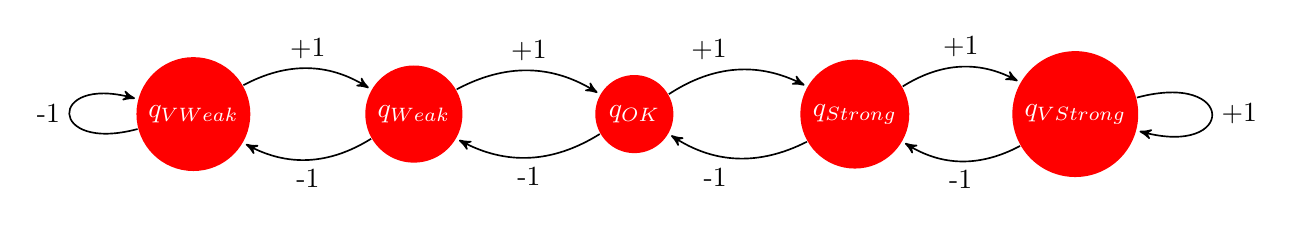
\begin{tikzpicture}[->,>=stealth',shorten >=1pt,auto,node distance=2.8cm,
                    semithick]
  \tikzstyle{every state}=[fill=red,draw=none,text=white]

  \node[state]         (A)                    {$q_{VWeak}$};
  \node[state]         (B) [right of=A]       {$q_{Weak}$};
  \node[state]         (C) [right of=B]       {$q_{OK}$};
  \node[state]         (D) [right of=C]       {$q_{Strong}$};
  \node[state]         (E) [right of=D]       {$q_{VStrong}$};

  \path (A) edge [bend left]  node {+1} (B)
                 edge [loop left]   node {-1}  (A) 
           (B) edge [bend left]  node {-1}  (A)
                 edge [bend left]  node {+1} (C)
           (C) edge [bend left]  node {-1}  (B)
                 edge [bend left]  node {+1} (D)
           (D) edge [bend left]  node {-1}  (C)
                 edge [bend left]  node {+1} (E)
           (E) edge [loop right] node {+1} (E)
                 edge [bend left]  node {-1}  (D);
\end{tikzpicture}




%% ==============================
\section{Evolution{\"a}rer Algorithmus}
%% ==============================

In diesem Abschnitt werden die Komponenten meines Algorithmus beschrieben, \dots

Im folgenden Abschnitt werden die folgenden Komponenten beschrieben, die f{\"u}r einen Evolution{\"a}ren Algorithmus verwendet werden. Dabei wurden die grundlegenden Bestandteile eines Evolution{\"a}ren Algorithmus beachtet und umgesetzt. 

\paragraph*{Signal}
Der wichtigste Bestandteil des Algorithmus ist das Individuum, dass in diesem Fall ein Signal ist. Ein Signal bildet eine Vibration ab. 
Das bedeutet es besitzt Attribute, die die L{\"a}nge der Vibration und die St{\"a}rke einer Vibration repr{\"a}sentieren.




%% ==============================
\section{Notizen}
%% ==============================
\label{ch:Entwurf:sec:Notizen}

Beim Entwurf, ok so wurde der Evolution{\"a}re Algorithmus aufgebaut.

Im Studiendesign w{\"u}rde der Ablauf und die Durchf{\"u}hrung aufgeschrieben.
Im Studiendesign sah die GUI so aus. 

Im Entwurf kannst du schreiben, dass die GUI so und so funktioniert und die Benutzerf{\"u}hrung ist so, da kann man noch ein sch{\"o}nes Diagramm zu machen zum Benutzerfluss (also ein Benutzerflussdiagramm) 

Oder im Studiendesign kann man das endg{\"u}ltige Benutzerflussdiagramm hinzuf{\"u}gen und Sagen ok wir hatten eine GUI denn das ist ja 1 zu 1 mein Studien design, so wie sich mein Nutzer in der GUI durchgeklickt, ist wie ich die Studie designed habe. Daher passt es super ins Studiendesign hinein, das klassische, ich hab das mit so und so vielen Leuten gemacht, so viele waren m{\"a}nnlich, so viele weiblich, alter, durchschnitt Standardabweichung, hab das an drei verschiedenen orten gemacht, Probanden waren bekannte freunde und {\"u}ber mailing listen sample of convenience. Das Prozedere ging so, die Leute sind gekommen, ich hab es ihnen erkl{\"a}rt, die haben das Armband angelegt, habe denen das erst einmal alleine abgespielt, die haben das Armband angelegt, haben am ende noch eine email hinterlassen um am Gewinnspiel teilzunehmen,

Und dann der Teil mit der Evaluierung, also das mit den Ergebnissen.

Tortendiagramm ist nicht sch{\"o}n, so und so viele bezeichnen sich als als musikalisch, Prozentzahlen reichen 
Bla fasel\ldots

%% ==============================
\section{Zusammenfassung}
%% ==============================
\label{ch:Entwurf:sec:zusammenfassung}

Am Ende sollten ggf. die wichtigsten Ergebnisse nochmal in \emph{einem}
kurzen Absatz zusammengefasst werden.

%%% Local Variables: 
%%% mode: latex
%%% TeX-master: "diplarb"
%%% End: 
